\documentclass[a4paper]{article}
\usepackage[utf8]{inputenc}
\usepackage[T1]{fontenc}
\usepackage[top=3cm, bottom=3cm, left=3cm, right=3cm]{geometry}
\usepackage{graphicx}
\usepackage[english]{babel}
\usepackage{tocloft}
\usepackage{amsmath}
\usepackage{mathtools}
\renewcommand{\cftsecleader}{\cftdotfill{\cftdotsep}}


\begin{document}
\begin{titlepage}

\addtolength{\voffset}{-1cm}
\title{ 
\linethickness{0.7mm}
\begin{center}
\line(1,0){400}\vspace{0.5cm}\\
\textbf{Visual motion disambiguation via contextual \\
		feedback control}
\line(1,0){400}\vspace{1cm}
\end{center}}
\author{Olivia Haas\thanks{LMU - Graduate school of Systemic Neurosciences - Munich, Germany}}
\date{}


\maketitle
\begin{center}
Supervisors:\\
\vspace{1mm}
Thomas Wachtler\\
\&\\
Christian Kellner\\

\vspace{0.5cm}
\begin{figure}[ht]
\centering

\includegraphics[scale=0.20]{BCCN}
\end{figure}
\vspace{0.5cm}

Lab Rotation\\
Martinsried (Munich, Germany)\\
\today\\

\vspace{0.1cm}
\begin{figure}[ht]
\centering

\includegraphics[scale=0.40]{GSN}
\end{figure}
\vspace{1cm}
\end{center}

\begin{abstract}

This lab rotation considered the affect of contextual feedback from the visual area MT to the primary visual cortex V1. Due to the aperture effect the movement of the presented square stimulus is amiguous accept at its edges. A model formulated to disambiguate the movement of each pixel consideres three stages within each model area. The first stage architecture is dominated by modulary feedback from the higher stage, whereas the second stage realizes an integration in space by an isotropic gaussian filter. Finally stage three normalizes estimations to emphasize unambgous signals.
\end{abstract}
\thispagestyle{empty}
\end{titlepage}

\newpage
\tableofcontents

\newpage
\section{Introcuction}
In a natrual environment the visual system deals with disambiguating moving stimuli. This process involves area V1 and MT of the dorsal stream, see Figure~\ref{fig:bouecke1}.\\

\vspace{0.5cm}
\begin{figure}[ht]
\centering
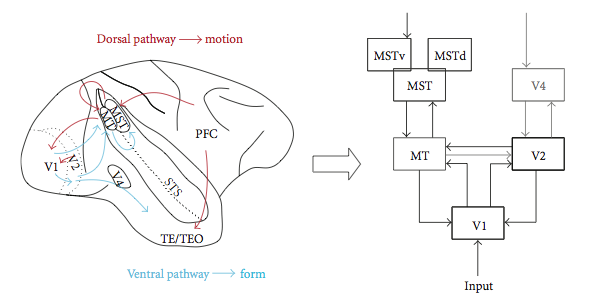
\includegraphics[width=11cm]{bouecke1}
\caption{The Dorsal pathway for motion processing. The location of involved brain areas are shown in the left part whereas a structural processing scheme is displayed on the right side.}
\label{fig:bouecke1}
\end{figure}
\vspace{0.5cm}


The input to model area V1 is considered to be the output of a local measure of motion, which is realized by the Reichard detector \cite{Reichard}. It delivers a movement orthogonal to an extended edge, which is known as the aperture problem. This can be resolved for localized image features, such as edges, but remains otherwise. Due to the small receptive field of single neurons a e.g. horizontal edge which is moving in a 45 degree agle seems to move upward instead.\\
Such an initial detection of motion can be contradicting within one object and remains to be resolved within following areas V1 and MT.\\
This disambiguation step is further subcategorized in six stages, three within the primary visual cortex and three in MT. Stages of both model areas are equal in their architecture.\\

\vspace{0.5cm}
\begin{figure}[ht]
\centering
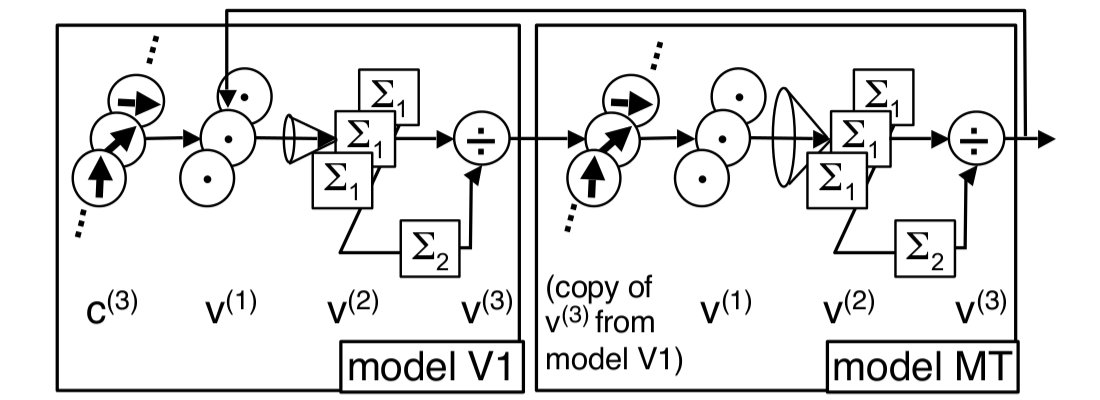
\includegraphics[width=11cm]{bayerl1}
\caption{Overview of the model architecture including three stages within area V1 and MT. Feedback stage $v^{(1)}$ is the output of area MT in V1 and zero in area MT, since no higher stages are considered to feed back to area MT. Stage $v^{(2)}$ consists of an integration with isotropic gaussian kernals in space realized by a convolution with the signal from $v^{(1)}$. $v^{(3)}$ is the lateral shunting inhibition stage ???? where unambiguous signals get amplified and amiguous ones get weakened.}
\label{fig:bayerl1}
\end{figure}
\vspace{0.5cm}

In order to solve the aperture problem this architecture involves feedforward and modulatory feedback, which provides a prediction mecanism and is realized via a recurrent loop, see Figure~\ref{fig:bayerl1}.\\
However, in V1 the fead forward signal from the reichard detector receives, as a first modulatory impact, feedback from area MT. The resulting actvity can then be interpreted as a measure of degree of match between the feedback and input at the next time step. Therefore, if the prediction of area MT matches the new input, the resulting activation will be maximal. The prupose of this step is to provide activations in V1 that match the expactations of the system\\
Further the resulting signal is sharpened by squaring it and then fead forward to the step of spatial integration. Here the signal from the previous step is convoluted with a two dimensional spatial gaussian. This serves the aim that motion information from neighbouring pixels are smoothened which can be compared to the vector average of the individual motion vectors. Here the model ensures integration of the surround into the motion information of each pixel which is then fead foreward to the final model area.\\
Here a normalization of movement direction estimations is realized by ?????

\section{Theory of Model Stages}
\subsection{Input Stage}
As a stimulus a black square on a white backround was used, which moves in the direction of $45^{\circ}$ with a step size of $\Delta t$.

\vspace{0.5cm}
\begin{figure}[ht]
\centering
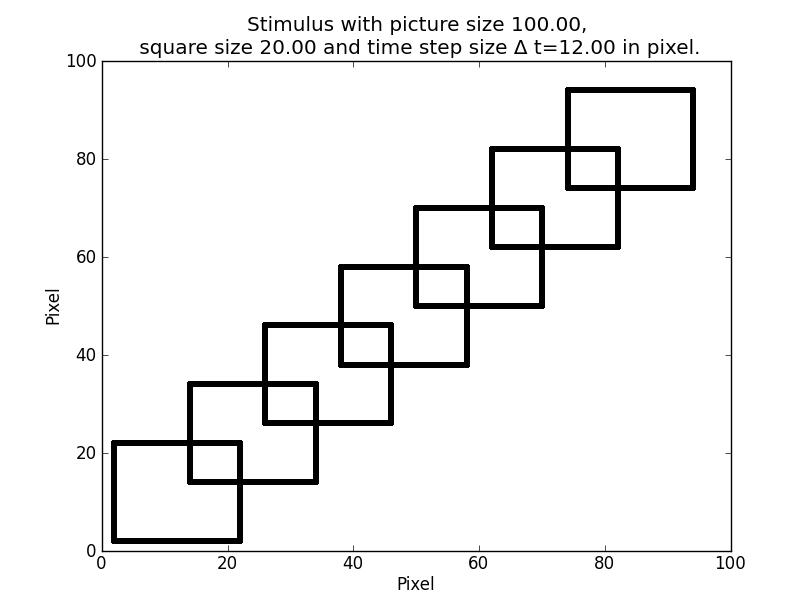
\includegraphics[width=8cm]{pics/stimulus}
\caption{Black square stimulus moving in the direction of 45 $^{\circ}$}. Each time step $\Delta t$ is represented as a single square at a certain position. For illustration reasons in this figure all time steps are presented together.
\label{fig:stimulus}
\end{figure}
\vspace{0.5cm}

As described above the input to model area V1 is the output of the Reichard detector.
In this lab rotation the reichard detector was not implemented as such but its output was created manually instead.\\
More explicit this means that for each pixel a population code was build to mimic the Reichard detector output. This was done by choosing 8 neurons which are individually tuned, in a gaussian fashion, to a certain angle in space. The neuronal tuning curves were chosen to equally divide the entire space (360$^{\circ}$) and can be seen in figure~\ref{fig:neuronGauss}

\vspace{0.5cm}
\begin{figure}[ht]
\centering
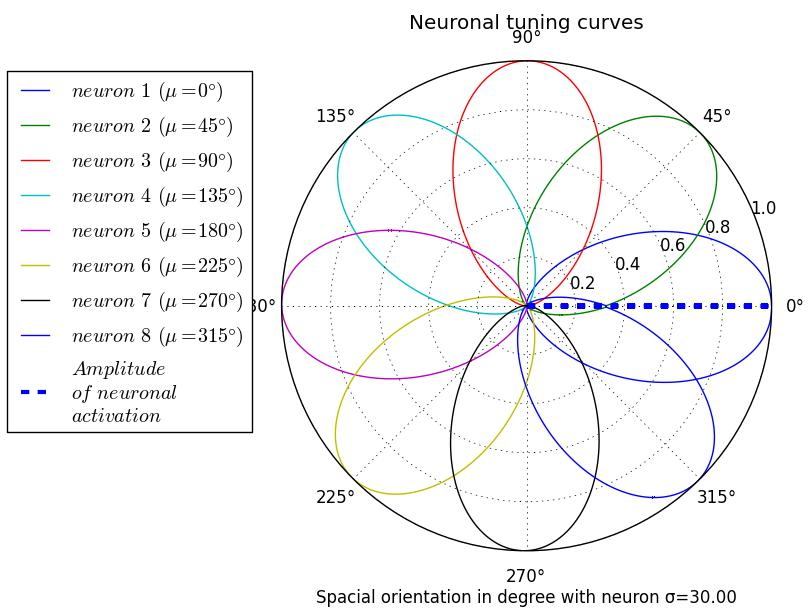
\includegraphics[width=8cm]{pics/neuronGauss}
\caption{Gaussian tuning curves in space of 8 different neurons with a maximal Amplitude of 1.}
\label{fig:neuronGauss}
\end{figure}
\vspace{0.5cm}

For each direction in space one can now write an eight dimensional vector, where the rows correspond to the individual neuron with its activation for the chosen direction in space (see figure~\ref{fig:neuronGauss}).\\
Due to the aperture problem we assume vertical vectors for horizontal stimulus edges and horizontal vectors for vertical edges. The three pixels which form the stimulus corners indecate the correct direction of 45$^{\circ}$.\\
In order to plot such a vector for each pixel $(x,y)$, the neuronal activation from the population code needs to be translated. This can be done by mutiping the eight dimensional vector containing the activation of the single neurons ($A(n)$) with its basis:

\begin{equation}
V=\left(A(1),A(2),\hdots, A(8)\right) \cdot \begin{pmatrix} (0&1) \\ (1&1)\\ \vdots\\ (-1&1)\end{pmatrix}
\label{vector1}
\end{equation}

To get the endpoints of the vector for the considered pixel, we sum each column of~\eqref{vector1}:

\begin{equation}
(\Delta x, \Delta y)=(\sum_{n=1}^{8}V(n,1),\sum_{n=1}^{8}V(n,2))
\label{vector2}
\end{equation}

Connecting the considered pixel $(x,y)$ with $(\Delta x, \Delta y)$ of quation~\eqref{vector2} draws the desired vector.\\
Repeating this procedure for all pixels gives us the final input ($in_{0}$) to the model (figure~\ref{fig:input}).

\vspace{0.5cm}
\begin{figure}[ht]
\centering
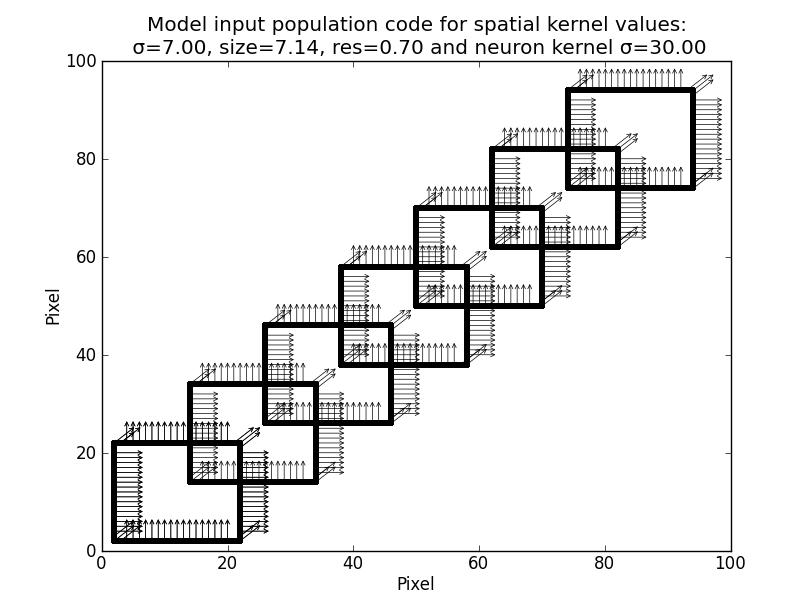
\includegraphics[width=8cm]{pics/input}
\caption{Input population codes with visualized vectors indecating the motion direction per pixel. One square represents one input per time step, moving in 45 $^{\circ}$.}
\label{fig:input}
\end{figure}
\vspace{0.5cm}

\subsection{Model stages}
All in- and outputs of model areas have the form of a population code ($(x,y,8)$), in order to store information for all pixels $(x,y)$ with activations of all 8 neurons per pixel.\\

\subsubsection{First Stage $S^{(1)}$}
Within the first model stage $S^{(1)}$ the input population code ($net_{IN}$) gets modified by the feedback ($net_{FB}$) fom the higher brain area. For model area V1 the feedback is the output of model area MT, which is moved to the current position of the stimulus. Model area MT however, does not receive feedback ($net_{FB}=0$) since no higher brain areas are considered in the model.\\
The modulation by the feedback enhances matching input signals, as shown in equation~\eqref{First_Stage}:

\begin{equation}
S^{(1)}=net_{IN}\cdot(1+100\cdot net_{FB})
\label{First_Stage}
\end{equation}

\subsubsection{Second Stage $S^{(2)}$}
The output of model stage $S^{(1)}$ is now fead foreward to stage two ($S^{(2)}$), where a convolution ($\star$) with a two dimensional, isotropic, spacial gaussian ($G^{x,space}$) enables a integration of neigbouring pixels in space and is comparable with its vector average.\\
In model area V1 this gaussian is replaced with the direc delta ($\sigma=0$), so that the convolutions equals the identity projection. In MT the guassian is normed to an Amplitude $A=1$ and has a kernal size of $\sigma=7$ and a resolution of $0.7$.\\
The spactial receptive field ratio of $V1:MT$ is $1:5$. The receptive field size of the reichard detector being $\sqrt{2\sigma^{2}}=1.41$ ($\sigma=1$) therefore inluences the receptive field size of MT to $\sqrt{1.41^{2}+7^{2}}=7.14$. With this we chose the total size of the two dimensional gaussian ($G^{x,space}$) to be $7.14$.
An example of such a gaussian $G^{x,space}$ can be seen in figure~\ref{fig:spatialGauss}:

\vspace{0.5cm}
\begin{figure}[ht]
\centering
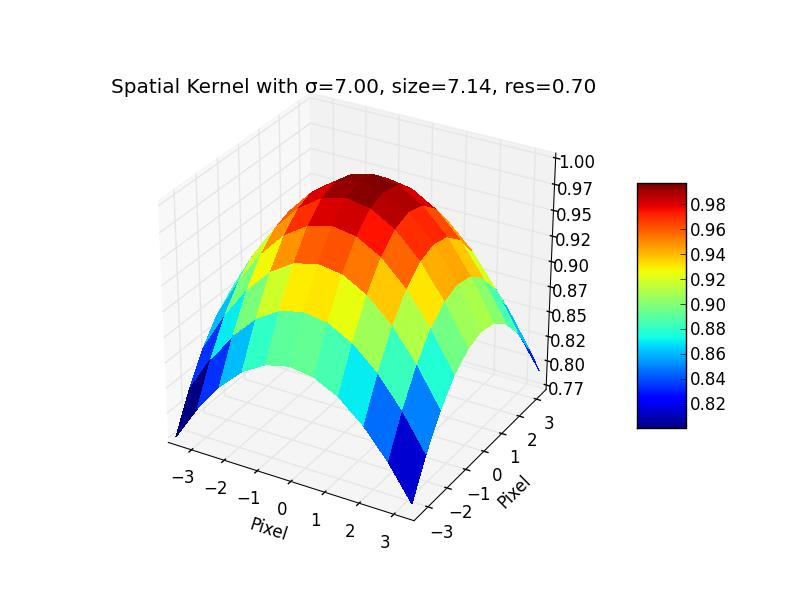
\includegraphics[width=8cm]{pics/spatialGauss}
\caption{Two dimensional Gauss used for the spactial convolution in~\eqref{Second_Stage}.}
\label{fig:spatialGauss}
\end{figure}
\vspace{0.5cm}

In equation~\eqref{Second_Stage} the convolution with such a spatial gaussian is shown. Also the input to this stage ($S^{(1)}$) is squared in order to sharpen the distribution.

\begin{equation}
S^{(2)}=(S^{(2)})^{2} \star G_{\sigma}^{x,space}
\label{Second_Stage}
\end{equation}

\subsubsection{Third Stage $S^{(3)}$}
The third stage gets the output of $S^{(2)}$ as input and serves the purpose to weaken ambigous signals, emphasize unambiguous signals and normalize direction estimations of previous stages.\\
This is done by weigthing the 8 dimensional vector of each pixel of the forwarded input $S^{(2)}$ by the global, 8 dimensional direction estimation $d$. Further it is then normalized by the maximum of the input population code ($max(S^{(2)})$).\\
Equation~\eqref{Third_Stage} illustrates this approach:

\begin{equation}
S^{(2)}=\frac{S^{(2)}\cdot d}{0.01+max(S^{(2)})}
\label{Third_Stage}
\end{equation}

\section{Results}

For a single time step ($\Delta t$) the three model stages discribed above are run for V1 and then MT, so that the output of one time step equals the output of MT.\\
The following overview (~\eqref{overview}) corresponds to one loop through figure~\ref{fig:bayerl1} where its output $S^{(3)}(MT)$ will be made to the following feedback.

\begin{equation}
\underbrace{S^{(1)}_{V1}\rightarrow S^{(2)}_{V1}\rightarrow S^{(3)}_{V1}\rightarrow S^{(1)}_{MT}\rightarrow S^{(2)}_{MT}\rightarrow S^{(3)}_{MT}}_{= 1 \cdot \Delta t}
\label{overview}
\end{equation}

The corresponding parameters are summarized in table~\ref{tab:variables}:

\begin{table}[ht]
\centering
\begin{tabular}{l|c c c}
	Model area & $net_{IN}$ & $net_{FB}$ & Spatial Kernal Size $\sigma$\\ \hline \hline\\
	V1 		  & $in_{0}$ & $S(x+\Delta x,y+\Delta y)^{(3)}_{MT}$ & 0 (dirac) \\ \\
	MT 		  & $S^{(3)}_{V1}$ & 0 & 7\\
\end{tabular}
\caption{Variables for model stages $S^{(1)}-S^{(3)}$ for both model areas, V1 and MT. $S(x+\Delta x, y+\Delta y)^{(3)}$ stands for the moved population code $S^{(3)}$ to the position of the next imput.}
\label{tab:variables}
\end{table}

Adoping the discribed model architecture, figure~\ref{fig:output} shows 7 time steps $\Delta t$ with vectors which correspond to the respective $S^{(3)}_{MT}$.

\vspace{0.5cm}
\begin{figure}[ht]
\centering
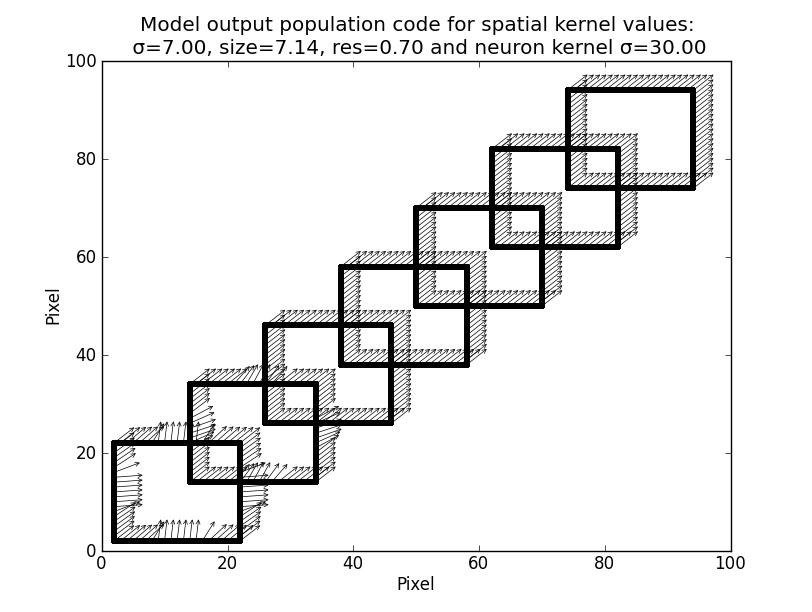
\includegraphics[width=8cm]{pics/output}
\caption{Outputs of 7 model time steps $\Delta t$ are shown where only the relevant vectors on the stimulus edges are presented.}
\label{fig:output}
\end{figure}
\vspace{0.5cm}

The feedback $net_{FB}$ which corresponds to the moved output of the pevious loop can be seen in figure~\ref{fig:feedback}. The first square does not have any corresponding vectors, since the first model loop does not have any feedback from previous loops.
\newpage
\begin{figure}[ht]
\centering
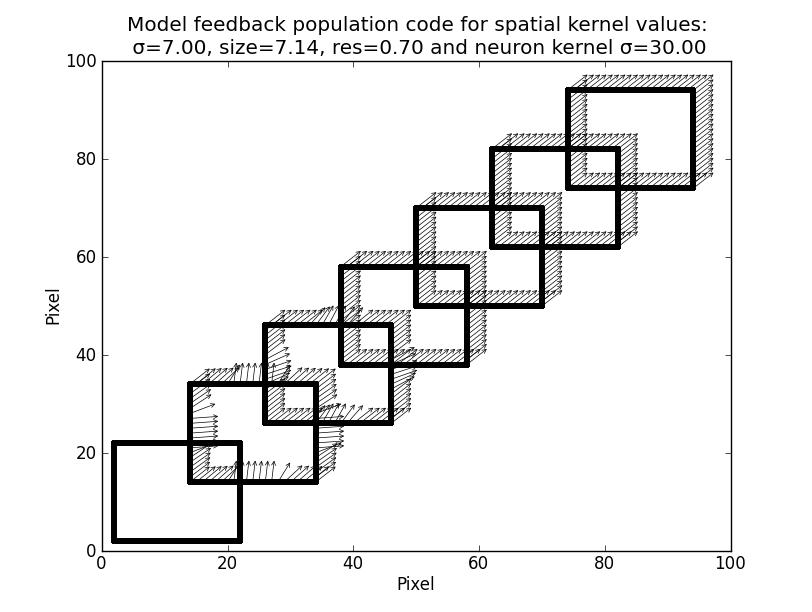
\includegraphics[width=8cm]{pics/feedback}
\caption{feedback of 7 model time steps $\Delta t$ are shown where only the relevant vectors on the stimulus edges are presented.}
\label{fig:feedback}
\end{figure}
\vspace{0.5cm}

To illustrate the most extreme cases, one can observe vectors in the middle of the horizontal and vertical stimulus edge. Due to their location being most distant from the unambiguous stimulus corners, their direction will unambiguate the slowest.\\







\end{document}